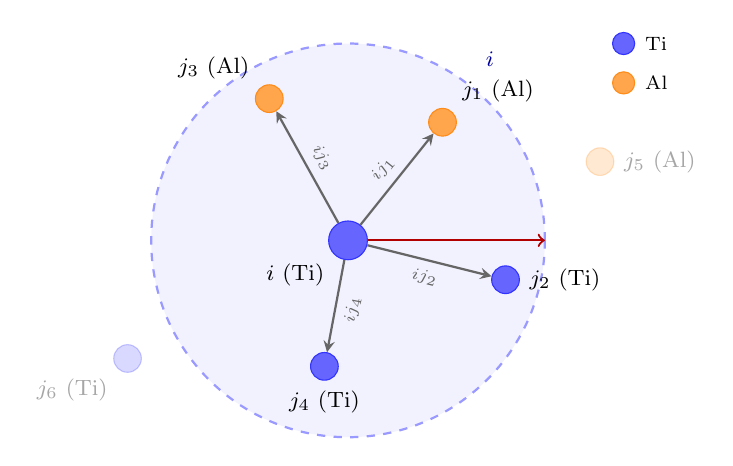
\begin{tikzpicture}[
    x=1cm, y=1cm,
    ti/.style={circle, fill=blue!60, draw=blue!80, minimum size=10pt, inner sep=0pt},
    al/.style={circle, fill=orange!70, draw=orange!90, minimum size=10pt, inner sep=0pt},
    outside/.style={opacity=0.25},
    rij/.style={->, >=stealth, thick, black!60},
    rij-label/.style={font=\footnotesize, midway},
]

% Cutoff circle
\draw[dashed, thick, blue!40, fill=blue!5] (0,0) circle (2.5cm);

% Cutoff radius annotation
\draw[<->, thick, red!70!black] (0,0) -- node[above, font=\footnotesize, red!70!black] {$\Rcut$} (2.5,0);

% Central atom i
\node[ti, minimum size=14pt, label={[font=\footnotesize]below left:$i$ (Ti)}] (center) at (0,0) {};

% Neighbors inside cutoff
\node[al, label={[font=\footnotesize]above right:$j_1$ (Al)}] (j1) at (1.2,1.5) {};
\node[ti, label={[font=\footnotesize]right:$j_2$ (Ti)}] (j2) at (2.0,-0.5) {};
\node[al, label={[font=\footnotesize]above left:$j_3$ (Al)}] (j3) at (-1.0,1.8) {};
\node[ti, label={[font=\footnotesize]below:$j_4$ (Ti)}] (j4) at (-0.3,-1.6) {};

% Atoms outside cutoff (grayed out)
\node[al, outside, label={[font=\footnotesize, opacity=0.35]right:$j_5$ (Al)}] (j5) at (3.2,1.0) {};
\node[ti, outside, label={[font=\footnotesize, opacity=0.35]below left:$j_6$ (Ti)}] (j6) at (-2.8,-1.5) {};

% Relative position vectors r_ij
\draw[rij] (center) -- node[rij-label, above, sloped] {$\relPos_{i j_1}$} (j1);
\draw[rij] (center) -- node[rij-label, below, sloped] {$\relPos_{i j_2}$} (j2);
\draw[rij] (center) -- node[rij-label, above, sloped] {$\relPos_{i j_3}$} (j3);
\draw[rij] (center) -- node[rij-label, below, sloped] {$\relPos_{i j_4}$} (j4);

% Neighborhood label
\node[font=\footnotesize, blue!60!black] at (1.8,2.3) {$\neigh{i}$};

% Legend
\node[ti, minimum size=8pt, label={[font=\scriptsize]right:Ti}] at (3.5,2.5) {};
\node[al, minimum size=8pt, label={[font=\scriptsize]right:Al}] at (3.5,2.0) {};

\end{tikzpicture}
